%%%%%%%%%%%%%%%%%%%%%%%%%%%%%%%%%%%%%%%%%
% Dreuw & Deselaer's Poster
% LaTeX Template
% Version 1.0 (11/04/13)
%
% Created by:
% Philippe Dreuw and Thomas Deselaers
% http://www-i6.informatik.rwth-aachen.de/~dreuw/latexbeamerposter.php
%
% This template has been downloaded from:
% http://www.LaTeXTemplates.com
%
% License:
% CC BY-NC-SA 3.0 (http://creativecommons.org/licenses/by-nc-sa/3.0/)
%
%%%%%%%%%%%%%%%%%%%%%%%%%%%%%%%%%%%%%%%%%

%----------------------------------------------------------------------------------------
%	PACKAGES AND OTHER DOCUMENT CONFIGURATIONS
%----------------------------------------------------------------------------------------

\documentclass[final,hyperref={pdfpagelabels=false}]{beamer}

\usepackage[orientation=landscape,size=a0,scale=1.3]{beamerposter} % Use the beamerposter package for laying out the poster with a portrait orientation and an a0 paper size

\usetheme{I6pd2} % Use the I6pd2 theme supplied with this template

\usepackage[english]{babel} % English language/hyphenation

\usepackage{amsmath,amsthm,amssymb,latexsym} % For including math equations, theorems, symbols, etc

\usepackage{tikz}

%\usepackage{times}\usefonttheme{professionalfonts}  % Uncomment to use Times as the main font
%\usefonttheme[onlymath]{serif} % Uncomment to use a Serif font within math environments

%\boldmath % Use bold for everything within the math environment

\usepackage{booktabs} % Top and bottom rules for tables

%\graphicspath{{figures/}} % Location of the graphics files

\usecaptiontemplate{\small\structure{\insertcaptionname~\insertcaptionnumber: }\insertcaption} % A fix for figure numbering

\newcommand{\bunderline}[1]{\underline{#1}}
\renewcommand{\vec}[1]{{\bunderline{#1}}}
\newcommand{\mat}[1]{{\bunderline{\bunderline{#1}}}}

\newcommand{\inred}[1]
        {\mbox{\color{red} #1}}
\newcommand{\inblu}[1]
        {\mbox{\color{blue} #1}}
\newcommand{\ingrn}[1]
        {\mbox{\color{green} #1}}
\newcommand{\inmag}[1]
        {\mbox{\color{magenta} #1}}
\newcommand{\inwhite}[1]
        {\mbox{\color{white} #1}}
\newcommand{\incyan}[1]
        {\mbox{\color{cyan} #1}}
\newcommand{\mbf}[1]{\text{\mbox{\boldmath $ #1 $}}}

\newcommand{\M}{\mathcal M}
\newcommand{\En}{\mathcal E}

%----------------------------------------------------------------------------------------
%	TITLE SECTION 
%----------------------------------------------------------------------------------------

\title{Towards Efficient Multiscale Numerical \\[0.75ex] Methods for Kinetic Models of Gases} % Poster title

\author{James A. Rossmanith and Lopamudra Palodhi} % Author(s)

\institute{Department of Mathematics, Iowa State University, 411 Morrill Road, Ames, Iowa, 50011, USA
  } % Institution(s)

%----------------------------------------------------------------------------------------
%	FOOTER TEXT
%----------------------------------------------------------------------------------------

\newcommand{\leftfoot}{\url{http://www.public.iastate.edu/~rossmani}} % Left footer text
\newcommand{\middlefoot}{Supported in Part by NSF Grant DMS--1620128} % Middle footer text
\newcommand{\rightfoot}{\url{rossmani@iastate.edu}} % Right footer text

%----------------------------------------------------------------------------------------

\begin{document}

\addtobeamertemplate{block end}{}{\vspace*{2ex}} % White space under blocks

\begin{frame}[t] % The whole poster is enclosed in one beamer frame

\begin{columns}[t] % The whole poster consists of two major columns, each of which can be subdivided further with another \begin{columns} block - the [t] argument aligns each column's content to the top

\begin{column}{.02\textwidth}\end{column} % Empty spacer column

\begin{column}{.31\textwidth} % The first column


%----------------------------------------------------------------------------------------
\begin{block}{Motivation: Many Real-World Problems are Multiscale}

\begin{figure}
\begin{center}
   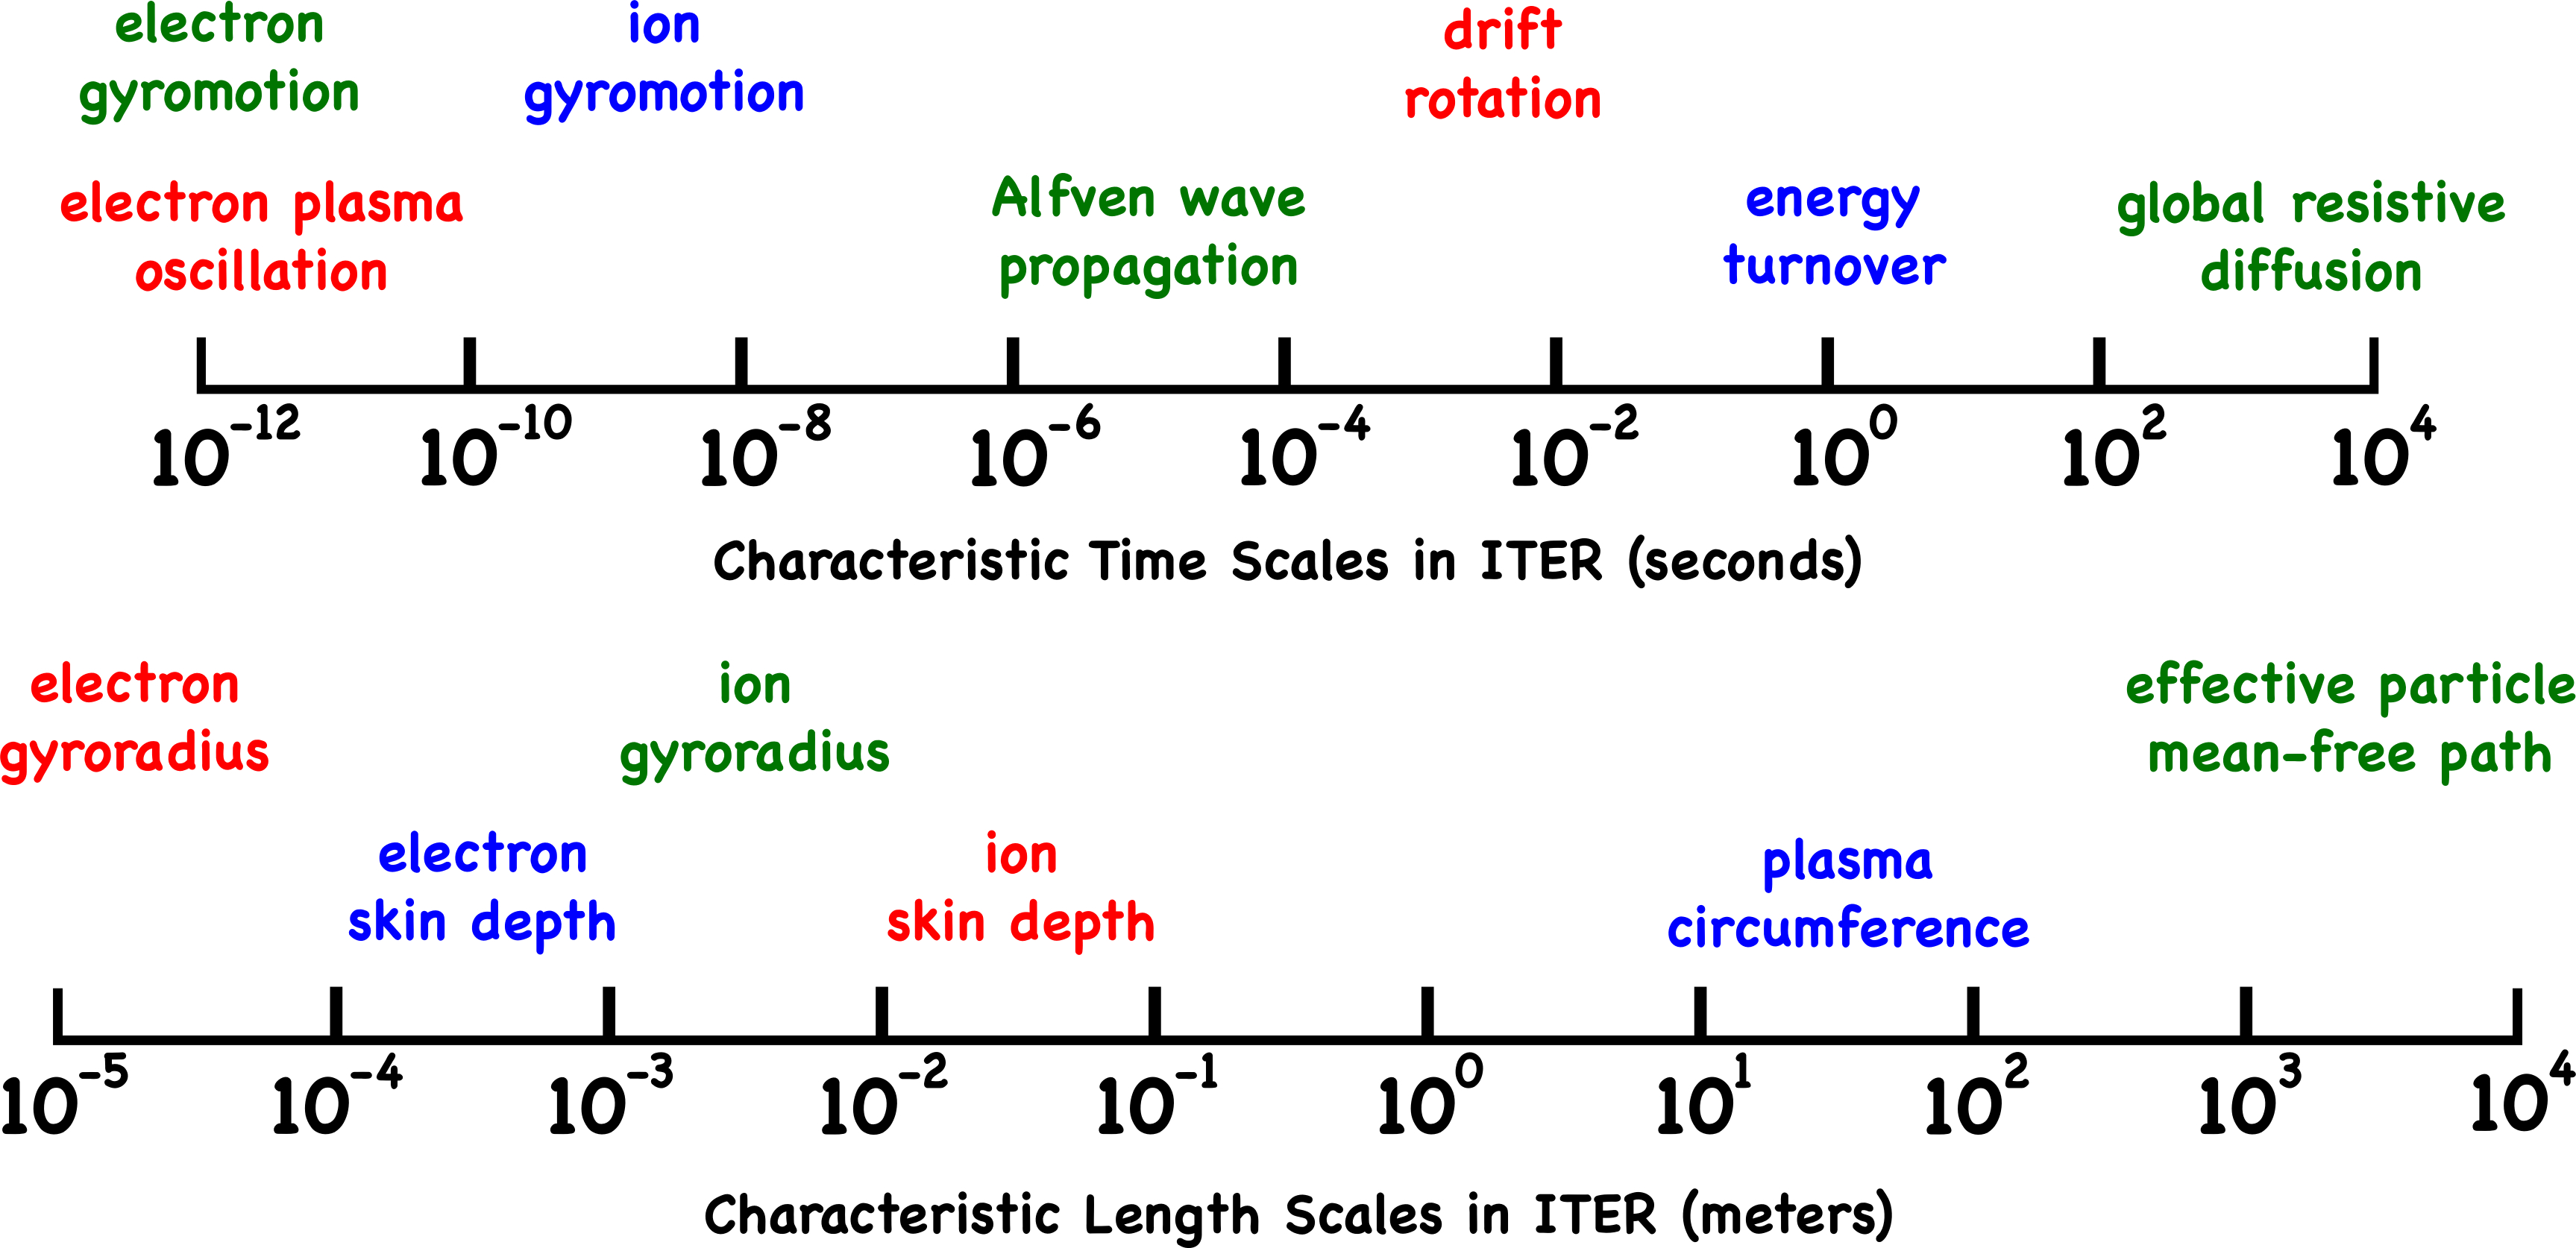
\includegraphics[height=150mm]{plasma_scales.jpg}
   \end{center}
\end{figure}

\vspace{-3mm}

\begin{itemize}
%\item Example from plasma physics
\item {\bf ITER}: effort to develop largest tokamak for magnetic confined fusion
\item Nonlinear effects couple many of the space/time scales,
	stiff PDEs
\item {\bf Goal}: develop multiscale methods (\inred{\bf Microscale} vs. \inred{\bf Macroscale})
\end{itemize}

\end{block}
%----------------------------------------------------------------------------------------

%----------------------------------------------------------------------------------------
\begin{block}{What We Consider the Microscale: Boltzmann's Equation}

\begin{center}
\begin{tabular}{ccc}
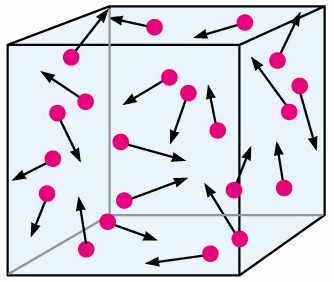
\includegraphics[height=110mm]{gas_particles.jpg} & \hspace{5mm} &
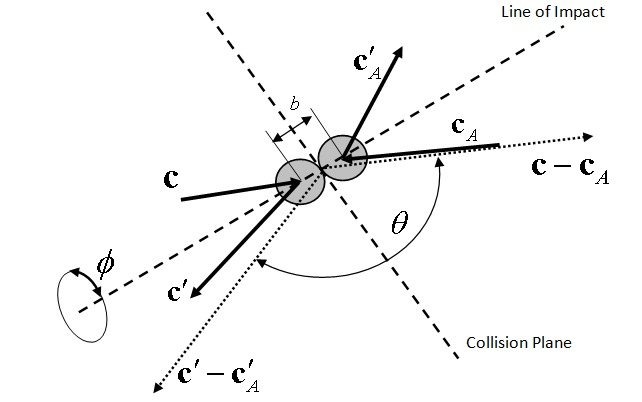
\includegraphics[height=110mm]{collisions.jpg}
\end{tabular}
\end{center}

\begin{itemize}
\item Hamiltonian:
\[
	{\mathcal H} = \underset{\inred{Kinetic}}{\underbrace{\frac{1}{2} \sum_{i=1}^{N} \vec{v}_i \cdot \vec{v}_i}}
	+ \underset{\inmag{External}}{\underbrace{\sum_{i=1}^{N} 
	\mathcal{V}\left( \vec{x}_i \right)}}
	+ \underset{\inblu{2-Body}}{\underbrace{\sum_{i=1}^{N}
	\sum_{j=1}^{N} 
	\mathcal{U}\left( \vec{x}_i - \vec{x}_j \right)}}
\]

%\vspace{-1mm}

\item Hamiltonian dynamics (for $j=1,2,\ldots,N$):
\[
	\dot{\vec{v}}_j = - {\mathcal H}_{,\vec{x}_j} \qquad \text{and} \qquad
	\dot{\vec{x}}_j =  {\mathcal H}_{,\vec{v}_j}
	= \vec{v}_j
\]

%\vspace{-1mm}

\item {\bf Difficulty:} $N$ is very large, think Avogadro's number: 
$N \sim 10^{23}$

\item $n$-point distribution function:
\[
f_n = 
\frac{N!}{(N-n)!}
\int f\left(t,\vec{x}_1,\ldots,\vec{x}_N,\vec{v}_1,\ldots,\vec{v}_N \right) \,
	\prod_{i=n+1}^N d\vec{x}_i \cdots d\vec{v}_i
\]

%\item {\bf [Bogoliubov, Born, Green, Yvon, \& Kirkwood, 
%1935,  1946--1947]}:
%\begin{align*}
% %{\mathcal H}_1 &= \frac{1}{2} \vec{v} \cdot \vec{v} + {\mathcal V}(\vec{x}), \qquad
%\frac{\partial f_1}{\partial t} &+ \vec{v} \cdot \frac{\partial f_1}{\partial \vec{x}} - \frac{\partial {\mathcal H}_1}{\partial \vec{x}} \cdot \frac{\partial f_1}{\partial \vec{v}} \\ &= \int \frac{\partial {\mathcal U}(\vec{x} - \vec{x}_2)}{\partial \vec{x}} \cdot \frac{\partial f_2}{\partial \vec{v}}
%\left(t, \vec{x},\vec{x}_2,\vec{v},\vec{v}_2 \right) \, d\vec{x}_2 d\vec{v}_2
%\end{align*}

\item  {\bf [Bhatnagar--Gross--Krook, 1954]}
\begin{gather*}
\frac{\partial f_1}{\partial t} +
	\vec{v} \cdot \frac{\partial f_1}{\partial \vec{x}}
	- \frac{\partial {\mathcal H}_1}{\partial \vec{x}}
	 \cdot \frac{\partial f_1}{\partial \vec{v}} =
	 \frac{1}{\varepsilon} \left( {\mathcal M} - f_1 \right), \quad
	 {\mathcal M} = \frac{\rho}{\left(2 \pi T \right)^{\frac{3}{2}}}
	\exp\left[- \frac{ \| \vec{v} - \vec{u} \|^2}{2T} \right]
\end{gather*}

\end{itemize}

\end{block}
%----------------------------------------------------------------------------------------

\end{column} % End of the first column

\begin{column}{.02\textwidth}\end{column} % Empty spacer column

\begin{column}{.31\textwidth} % The second column

%----------------------------------------------------------------------------------------
\begin{block}{What We Consider the Macroscale: Compressible Euler Equations}

\begin{itemize}
\item $\varepsilon \rightarrow 0^+$, yields
the macroscale: \quad $f_1 \rightarrow {\mathcal M}$

\item In this limit, moments of ${\mathcal M}$ satisfy the compressible Euler equations:
\begin{gather*}
\frac{\partial}{\partial t} 
\begin{bmatrix} \rho \\ \rho \vec{u} \\ {\mathcal E} \end{bmatrix}
+
\vec{\nabla} \cdot
\begin{bmatrix} \rho \vec{u} \\ \rho \vec{u} \vec{u} + p {\mathbb I} \\ 
\vec{u} \left( {\mathcal E} + p \right) \end{bmatrix} = \begin{bmatrix} 
0 \\ - \rho {\mathcal H}_{1,\vec{x}} \\ -\rho \vec{u} \cdot {\mathcal H}_{1,\vec{x}}
\end{bmatrix}, \quad
{\mathcal E} = \frac{p}{\gamma - 1} + \frac{1}{2} \rho \| \vec{u} \|^2
\end{gather*}
\end{itemize}

\end{block}
%----------------------------------------------------------------------------------------

%----------------------------------------------------------------------------------------
\begin{block}{From the Macroscale to the Microscale via the Knudsen Number}

\begin{figure}
\begin{center}
   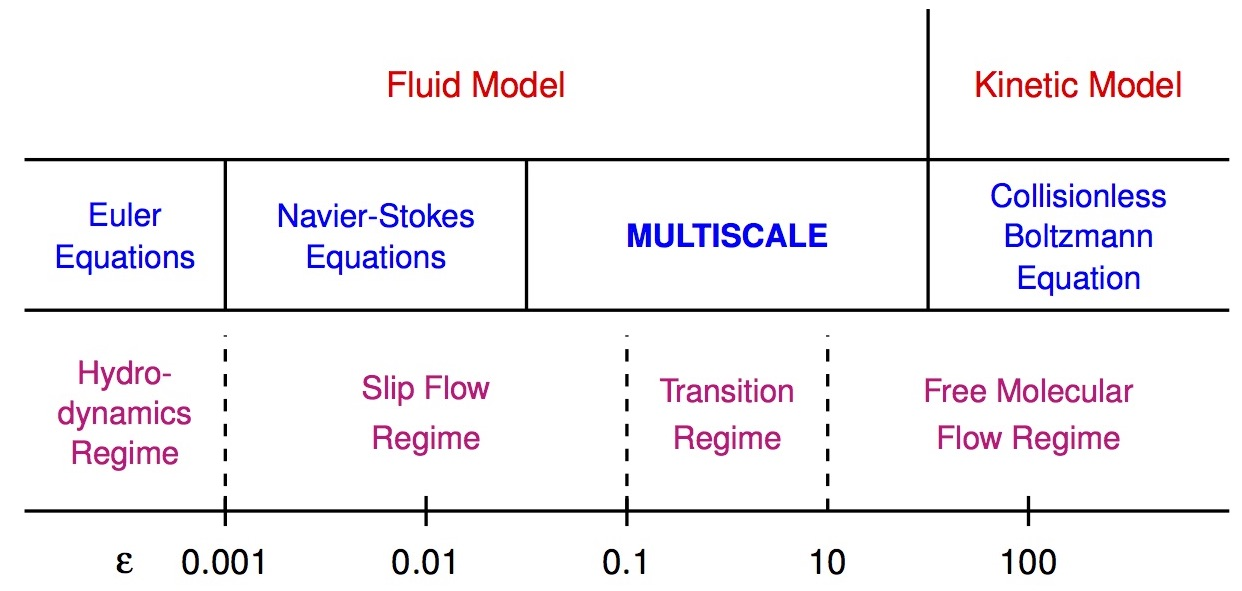
\includegraphics[height=140mm]{knudsen.jpg}
   \end{center}
\end{figure}

\vspace{-4mm}

\begin{itemize}

\item {\bf Knudsen number}: ratio of mean-free path to characteristic length scale

\item A multiscale solver should be able to efficiently bridge all of these scales 

\end{itemize}
     
\end{block}
%----------------------------------------------------------------------------------------

%----------------------------------------------------------------------------------------
\begin{block}{Key Concept: Asymptotic-Preserving (AP) {\bf [Jin, 1999 \& 2012]}
}

\begin{figure}
\begin{center}
   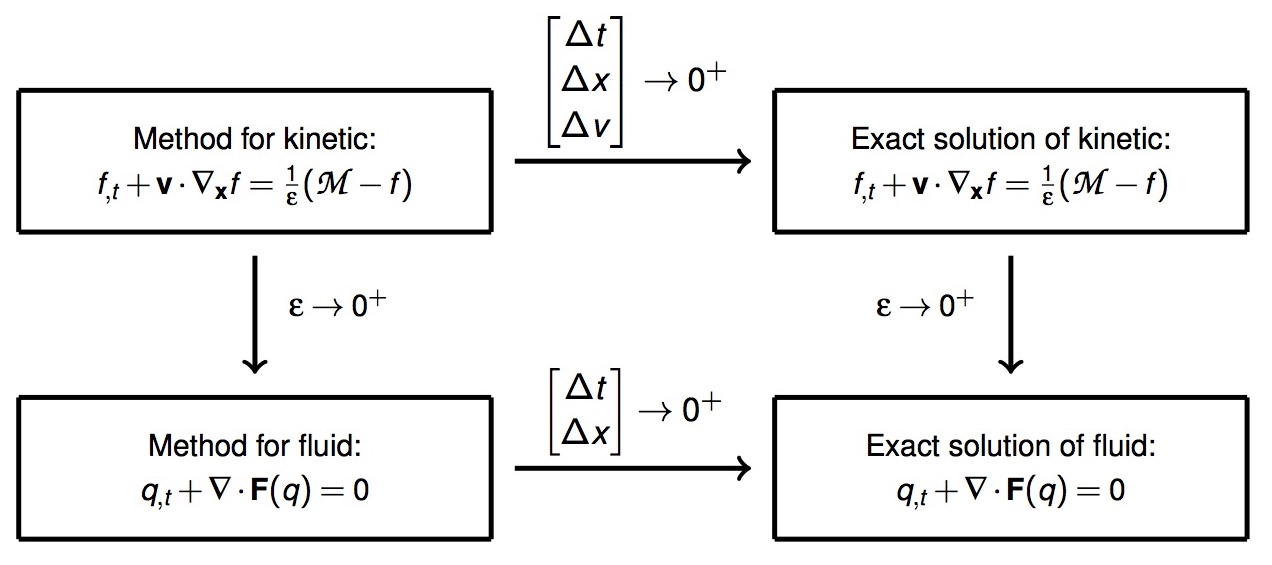
\includegraphics[height=120mm]{APdiagram.jpg}
   \end{center}
\end{figure}

%\vspace{-4mm}

%\begin{itemize}
%\item Popularized by {\bf [Jin, 1999 \& 2012]}
%\item AP is a necessary condition for efficiency in the limit $\varepsilon \rightarrow 0^+$
%\end{itemize}
     
\end{block}
%----------------------------------------------------------------------------------------

%----------------------------------------------------------------------------------------
\begin{block}{Approach \#1: Moment-Closure Methods}


\begin{itemize}

\item{\bf Moment equations:} (for simplicity, shown here in 1D)
\begin{gather*}
  M_{\ell} := \int_{-\infty}^{\infty} v^\ell f(t,x,v) \, dv \quad \text{and} \quad
  {\mathcal C}_{\ell} := \int_{-\infty}^{\infty} v^\ell {\mathcal C}(f) \, dv \\
  M_{\ell,t} + M_{\ell+1,x} = -\ell M_{\ell-1} {\mathcal H}_{1,x} + {\mathcal C}_{\ell}
\end{gather*}

\item How to close this system? {\bf [Grad, 1949]}, {\bf [Levermore, 1996]}, $\ldots$
%\item Imperfect options: {\bf [Grad, 1949]}, {\bf [Levermore, 1996]}, $\ldots$
\end{itemize}
     
\end{block}
%----------------------------------------------------------------------------------------


%----------------------------------------------------------------------------------------

\end{column} % End of the first column

\begin{column}{.02\textwidth}\end{column} % Empty spacer column
 
\begin{column}{.31\textwidth} % The third column


%----------------------------------------------------------------------------------------
\begin{block}{Approach \#2: AP Kinetic Schemes}


\begin{itemize}
\item A simple AP operator split scheme:
\begin{align*}
\inred{\text{Transport  step:}} & \quad f^{\star}_{ij} = f^{n}_{ij}  - \frac{\Delta t}{\Delta x}
\left[ v^+_j \left( f^{n}_{ij} - f^{n}_{i-1 \, j} \right)
+ v^-_j \left( f^{n}_{i+1 \, j} - f^{n}_{ij} \right) \right] \\
\inred{\text{Compute Maxwellian:}} & \quad
f^{\star} \quad \rightarrow \quad \left( \rho^{\star}, u^{\star}, p^{\star} \right)
\quad \rightarrow \quad {\mathcal M}^{\star} \\
\inred{\text{Collision  step:}} & \quad f^{n+1}_{ij} = \left( \frac{\varepsilon}{\varepsilon + \Delta t}
 \right) \, f^{\star}_{ij} + \left( \frac{\Delta t}{\varepsilon + \Delta t} \right) \, {\mathcal M}^{\star}_{ij}
\end{align*}

\item High-order extensions via WENO-IMEX {\bf [Pieraccini \& Puppo, 2008]}
%\begin{align*}
%f^{(1)} &= f^n + \frac{\Delta t}{\varepsilon} a_{11} \left( {\mathcal M}^{(1)}
%- f^{(1)} \right), \\
%f^{(s)} &= f^n - {\Delta t} \sum_{\ell=1}^{s-1} \tilde{a}_{s\ell} v f_{,x}^{(\ell)}
% + \frac{\Delta t}{\varepsilon} \sum_{\ell=1}^{s} a_{s\ell} \left( {\mathcal M}^{(\ell)}
%- f^{(\ell)} \right), \quad 2 \le s \le \nu, \\
%f^{n+1} &= f^n - {\Delta t} \sum_{s=1}^{\nu} \tilde{w}_s v f_{,x}^{(s)}
%+ \frac{\Delta t}{\varepsilon} \sum_{s=1}^{\nu} {w}_s \left( {\mathcal M}^{(s)} - 
%f^{(s)} \right).
%\end{align*}
\end{itemize}
     
\end{block}
%----------------------------------------------------------------------------------------

%----------------------------------------------------------------------------------------
\begin{block}{Approach \#3: Micro-Macro Decomposition Schemes}


\begin{itemize}
\item {\bf [Bennoune, Lemou, and Mieussens, 2008]} \& 
{\bf [Xiong \& Qiu, 2016]}:
\begin{gather*}
   f = \M + \varepsilon g \\
 \begin{bmatrix} \rho \\ \rho u \\ {\mathcal E} \end{bmatrix}_{,t} +
	 \begin{bmatrix} \rho u \\ \rho u^2 + p \\ u ({\mathcal E}+p) 
	 + \inred{$\frac{\varepsilon}{2} \langle v^3 g \rangle$} \end{bmatrix}_{,x} = 0, \quad \text{where} \quad
	 \En = \frac{1}{2} p + \frac{1}{2} u^2 \\
g_{,t} + \left( {\mathcal I} - 
\Pi_{\M} \right)\left( v g_{,x} \right) = -\frac{1}{\varepsilon} \Bigl[ 
g + \left( {\mathcal I} - 
\Pi_{\M} \right)\left( v \M_{,x} \right) \Bigr]
\end{gather*}

\item Orthogonal projector $\Pi_{\M} (\phi)$ onto Maxwellian distribution

\end{itemize}
     
\end{block}
%----------------------------------------------------------------------------------------

%----------------------------------------------------------------------------------------
\begin{block}{New approach: Moment-Closure + Micro-Macro Decomposition}


\begin{itemize}
\item Hermite expansion + Micro-Macro decomposition:
\begin{equation*}
%    f = \underbrace{\M}_\text{\inblu{Macroscopic}} + \underbrace{ \varepsilon \rho^{-1} \M
 %    \sum_{k=3}^{\infty} \alpha_k T^{-\frac{k}{2}} \psi_k\left( \frac{v - u}{\sqrt{T}} \right)}_{\text{\inred{Microscopic}}}
     f = \M + \varepsilon \rho^{-1} \M
     \sum_{k=3}^{\infty} \alpha_k T^{-\frac{k}{2}} \psi_k\left( v \right)
\end{equation*}
\item Wave propagation method for macro + RK-IMEX for micro:
%\begin{equation*}
%	\vec{\alpha}^{n+1} = \vec{\alpha}^{n} - \Delta t \, \mat{A}^{n+1} \, \vec{\alpha}^{n}_{,x} 
%	- \Delta t \, \mat{B}^{n+1} \, \vec{\alpha}^n  - \frac{\Delta t}{\varepsilon} \left( \vec{\alpha}^{n+1}
%	+ \vec{s}^{n+1} \right)
%\end{equation*}
\item {$\varepsilon=10^{-3}$ with only two modes ($\alpha_3$ and $\alpha_4$)}
\begin{center}
\begin{tabular}{cc}
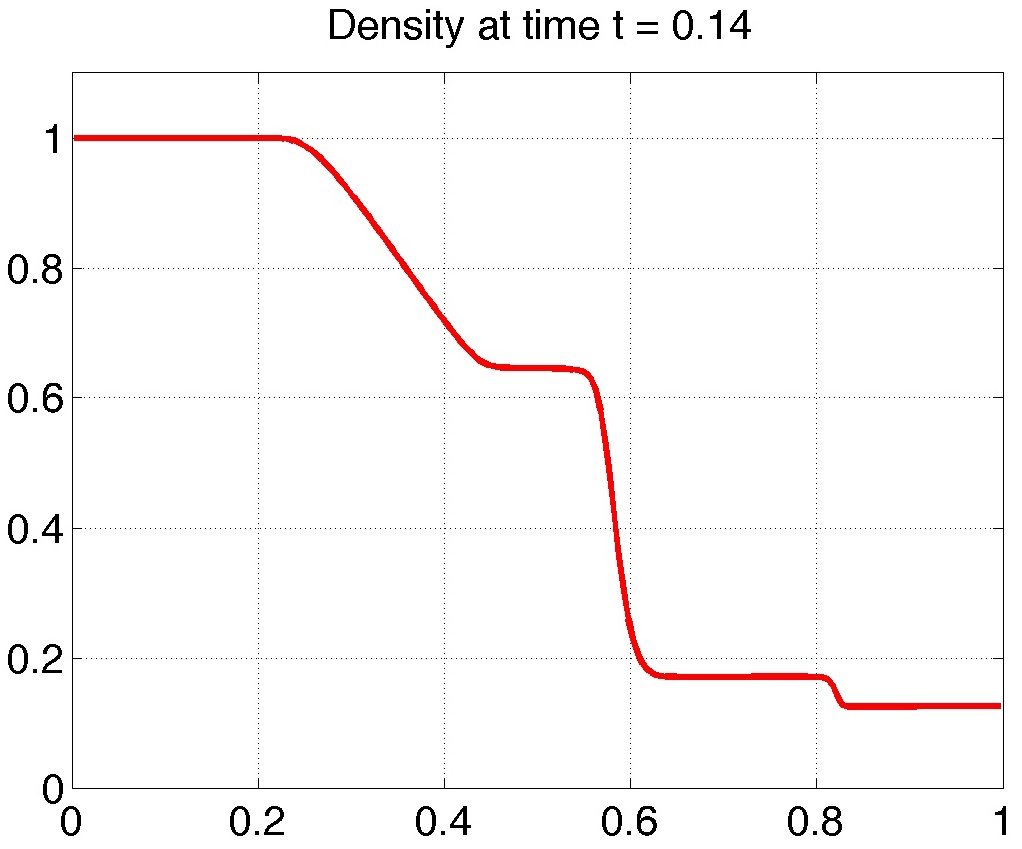
\includegraphics[width=110mm]{hbgk_density_1em3.jpg}  &
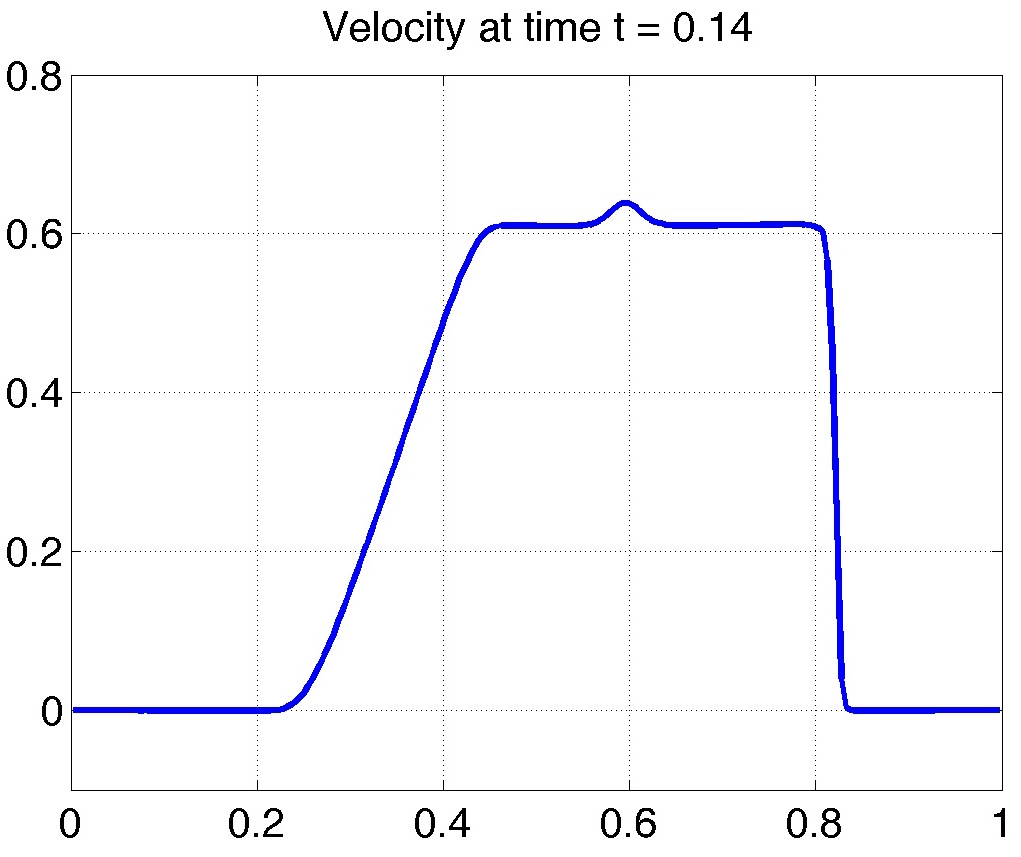
\includegraphics[width=110mm]{hbgk_velocity_1em3.jpg} \\
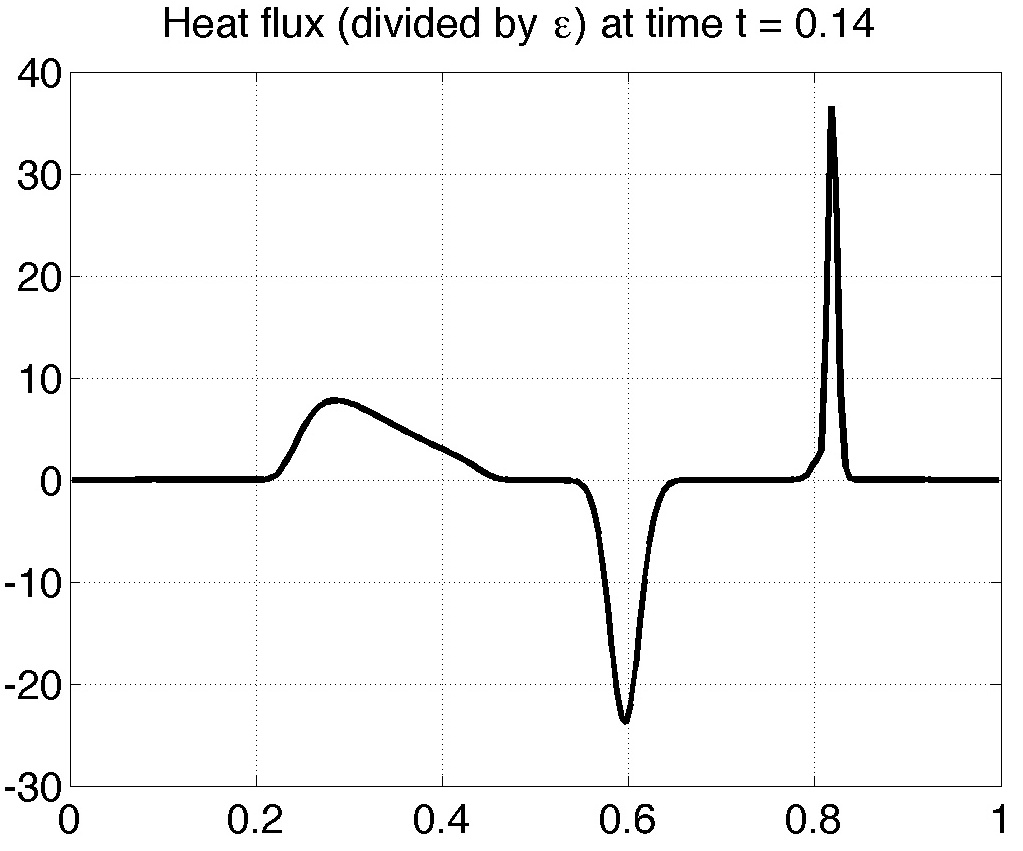
\includegraphics[width=110mm]{hbgk_heatflux_1em3.jpg} &
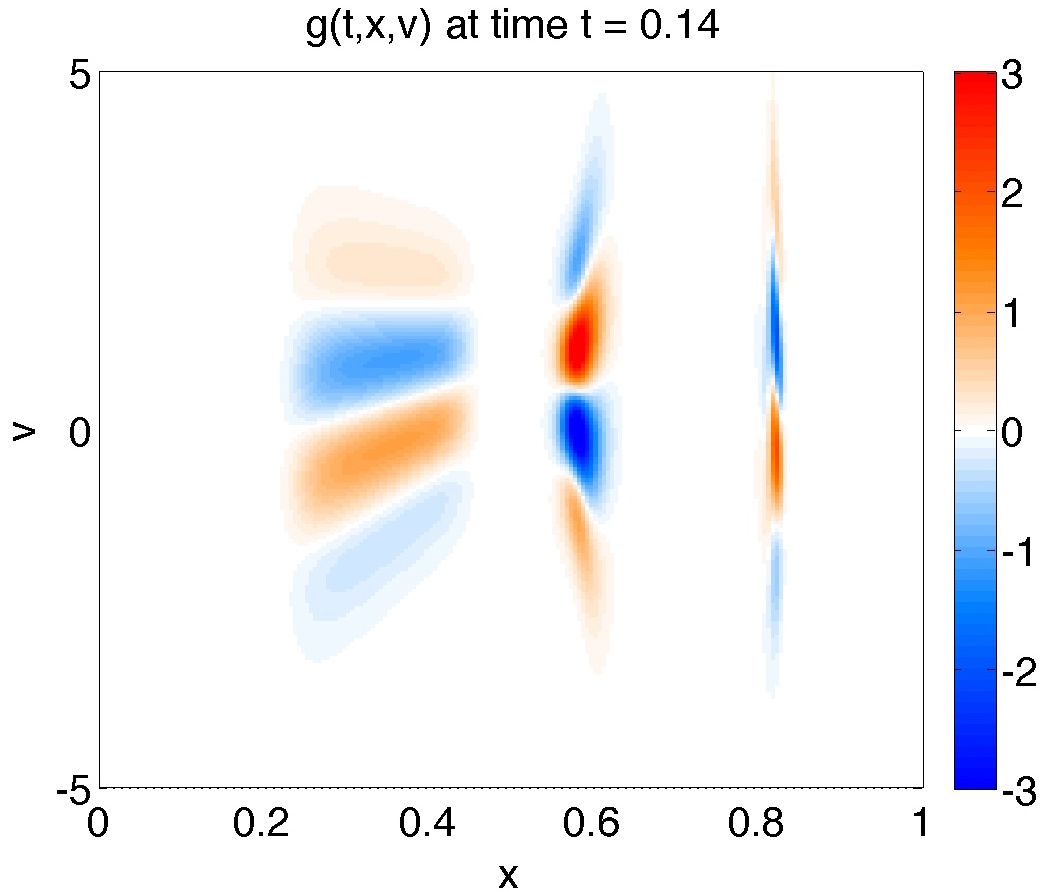
\includegraphics[width=110mm]{hbgk_g_1em3.jpg}
\end{tabular}
\end{center}
\end{itemize}
\end{block}
%----------------------------------------------------------------------------------------


\end{column} % End of the second column

\begin{column}{.015\textwidth}\end{column} % Empty spacer column

\end{columns} % End of all the columns in the poster

\end{frame} % End of the enclosing frame

\end{document}